%!TEX TS-program = xelatex
%!TEX encoding = UTF-8 Unicode

\documentclass[12pt]{extarticle}
% extarticle is like article but can handle 8pt, 9pt, 10pt, 11pt, 12pt, 14pt, 17pt, and 20pt text

\def \ititle {Origins of Mind}

\def \isubtitle {Lecture 01}

\def \iauthor {Stephen A. Butterfill}
\def \iemail{s.butterfill@warwick.ac.uk}
\date{}

%for strikethrough
\usepackage[normalem]{ulem}

\input{$HOME/Documents/submissions/preamble_steve_handout}

%\bibpunct{}{}{,}{s}{}{,}  %use superscript TICS style bib
%remove hanging indent for TICS style bib
%TODO doesnt work
\setlength{\bibhang}{0em}
%\setlength{\bibsep}{0.5em}


%itemize bullet should be dash
\renewcommand{\labelitemi}{$-$}

\begin{document}

\begin{multicols}{3}

\setlength\footnotesep{1em}


\bibliographystyle{newapa} %apalike

%\maketitle
%\tableofcontents




%---------------
%--- start paste



\def \ititle {Lecture 01}

\begin{center}

{\Large

\textbf{\ititle}

}



\iemail %

\end{center}



\section{The Question}

How do humans first come to know  about---and to knowingly manipulate---objects,
causes, words, numbers, colours, actions and minds?

‘... ’tis past doubt, that Men have in their Minds several Ideas, such as are those expressed by the words, Whiteness, Hardness, ... and others: It is in the first place to be enquired, How he comes by them?’
\citep[p.\ 104]{Locke:1975qo}

‘How does it come about that the development of organic behavior into controlled inquiry brings about the differentiation and cooperation of observational and conceptual operations?’
\citep[p.\ 12]{Dewey:1938yp}

‘the fundamental explicandum, is the organism and its propositional attitudes ... Cognitive psychologists accept ... the  ... necessity of explaining how organisms come to have the attitudes to propositions that they do.’
\citep[p.\ 198]{Fodor:1975pb}



\section{From Myths to Mechanisms}

‘the soul inherently contains the sources of various notions and doctrines which external objects merely rouse up on suitable occasions’
\citep[p.\ 48]{Leibniz:1996bl}

‘Men, barely by the Use of their natural Faculties, may attain to all the Knowledge
they have, without the help of any innate Impressions’
\citep[p.\ 48]{Locke:1975qo}

‘Developmental science [...] has shown that both these views are false’
\citep[p.\ 89]{Spelke:2007hb}.



\section{Davidson’s Challenge}

‘We have many vocabularies for describing nature when we regard it as mindless, and we have a mentalistic vocabulary for describing thought and intentional action; what we lack is a way of describing what is in between’ \citep[p.\ 11]{Davidson:1999ju}

\subsection{Uncomplicated Account of Minds and Actions}
For any given proposition [There’s a spider behind the book] and any given human [Wy]
...
\begin{enumerate}
\item Either Wy believes that there’s a spider behind the book, or she does not.
\item Either Wy can act for the reason that there is, or seems to be, a spider behind the book, or else she cannot.
\item The first alternatives of (1) and (2) are either both true or both false.
\end{enumerate}



\section{Unperceived Objects: An Illustration of Davidon's Challenge}

When do humans first come to know facts about the locations of objects they are not
perceiving?

\begin{center}
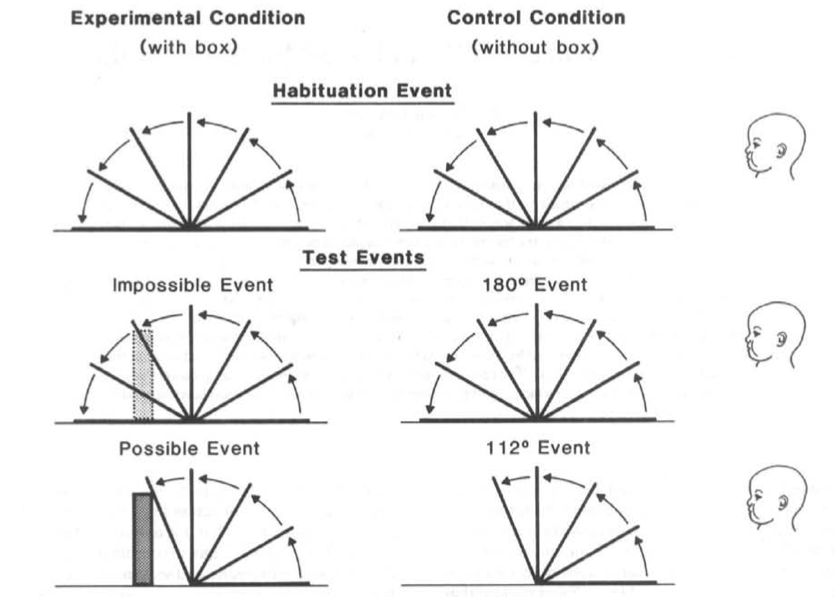
\includegraphics[scale=0.25]{img/baillargeon_1987_fig1.neg.png}
\end{center}
\begin{center} \citealp{baillargeon:1987_object} figure 1 \end{center}

\begin{center}
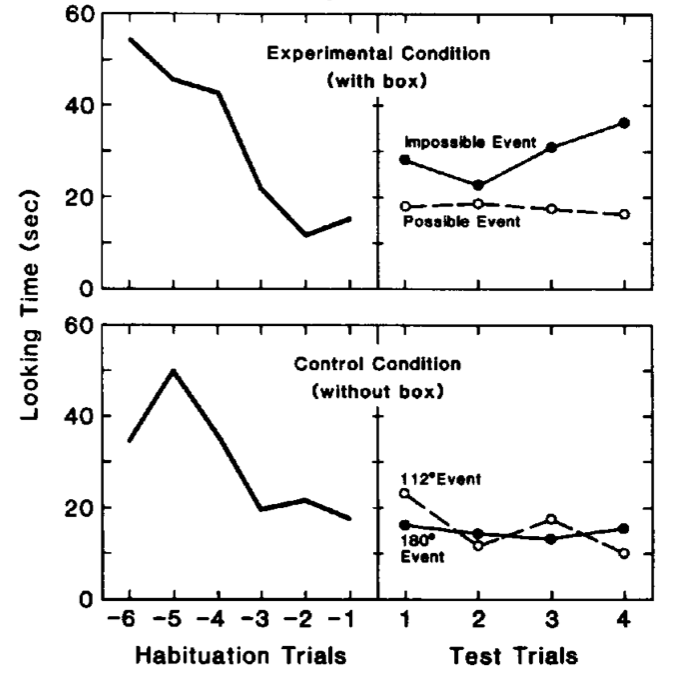
\includegraphics[scale=0.25]{img/baillargeon_1987_fig2.neg.png}
\end{center}
\begin{center} \citealp{baillargeon:1987_object} figure 2 \end{center}

‘action demands are not the only cause of failures on occlusion tasks’
\citep[p.\ 291]{shinskey:2012_disappearing}.

‘violation-of-expectation experiments, using looking-time measures, suggested that infants
have object permanence in occlusion conditions; but simplified-search studies confirm that
infants fail to reach towards occluded objects, suggesting that infants do not have object
permanence in occlusion conditions. This discrepancy, however, is only the tip of the
iceberg. Results of studies attempting to measure infants’ cognitive abilities using reaching
measures often contradict results gained while using looking-time measures.’
\citep[p.\ 994]{charles:2009_object}

‘there are many separable systems of mental representations ... the task ... is to ... [find] the distinct systems of mental representation and to understand their development and integration’
\citep[p.\ 1522]{Hood:2000bf}.

\textit{Object permanence}:
the ability to know facts about objects you aren't currently perceiving.



\section{Social Interaction: Acquiring Your First Words}

\subsection{A Conjecture}

‘humans acquire knowledge at a pace far outstripping that found in any other species.
Recent evidence indicates that interpersonal understanding ...
plays a pivotal role in this achievement.’
\citep[p.\ 40]{Baldwin:2000qq}

‘functions traditionally considered hallmarks of individual cognition originated through
the need to interact with others ...\ perception, action, and cognition are grounded in
social interaction.’
\citep[p.\ 103]{Knoblich:2006bn}

Vygotskian Intelligence Hypothesis:
‘the unique aspects of human cognition ... were driven by, or even constituted by,
social co-operation.’
\citep[p.\ 1]{Moll:2007gu}

‘human cognitive abilities ... [are] built upon social interaction’
\citep{sinigaglia:2008_roots} %*page

\subsection{How do children acquire words?}

‘we grasp the concept of truth only when we can communicate the
contents---the propositional contents---of the shared experience, and
this requires language’
\citep[p.\ 27]{Davidson:1997wj}.

‘The ability to discriminate, to act differentially in the face  of clues to the presence of food, danger or safety, is present in all animals and does not require reason.  Nor does the learning, even of complex routines, require reason, for it is possible to learn how to act without learning that anything is the case.’
\citep[p.\ 326]{Davidson:1982je}

‘A child learning to speak is learning habits and associations which are just as much determined by the environment as the habit of expecting dogs to bark and cocks to crow’
\citep[p.\ 71]{Russell:1921ww}

‘[t]he child learns this language from the grown-ups by being trained to its use. I am using the word ‘trained’ in a way strictly analogous to that in which we talk of an animal being trained to do certain things. It is done by means of example, reward, punishment, and suchlike’
\citep[p.\ 77]{Wittgenstein:1972lj}

‘the child’s early learning of a verbal response depends on society's reinforcement of the response in association with the stimulations that merit the response’
(\citep[p.\ 82]{Quine:1960fe}; compare \citep[pp.\ 28--9]{Quine:1974rd})

‘Before we have an idea of truth or error, before the advent of concepts or propositional thought,
there is a rudiment of communication in the simple discovery that sounds produce results. Crying is the first step toward language when crying is found to procure one or another form of relief or satisfaction. More specific sounds, imitated or not, are rapidly associated with more specific pleasures.
Here use //p. 71// would be meaning, if anything like intention and meaning were in the picture.
A large further step has been taken when the child notices that others also make distinctive sounds at the same time the child is having the experiences that provoke its own volunteered sounds.
For the adult, these sounds have a meaning, perhaps as one word sentences. The adult sees herself as doing a little ostensive teaching: “Eat,” “Red,” “Ball,” “Mamma,” “Milk,” “No.”

There is now room for what the adult views as error: the child says “Block” when it is a slab. This move fails to be rewarded, and the conditioning becomes more complex’
\citep[pp.\ 70--1]{Davidson:2000mt}

Children acquiring language create their own words before they learn to use those of the adults
around them.

‘From the time they first use words until they are about two or two-and-a-half,
children noticeably and systematically overextend words. For example, one child used
the word “apple” to refer to balls of soap, a rubber-ball, a ball-lamp, a tomato,
cherries, peaches, strawberries, an orange, a pear, an onion, and round biscuits’
\citep[p.\ 35]{Clark:1993bv}

Children can create their own languages
with no experience of others' languages
\citep{Kegl:1999es,Senghas:2001zm,Goldin-Meadow:2003pj}.




%--- end paste
%---------------

\footnotesize
\bibliography{$HOME/endnote/phd_biblio}

\end{multicols}

\end{document}
